\chapter{Secondary test of step response}\label{ap:drone_secondary_test}
The purpose of this test is to get a model of how the drone responds to a step in throttle, and to make a function describing this behaviour. The test will be performed in the Motion tracking lab, located at AAU Fredrik Bajers Vej 7 room C2-111, where the Vicon system \ref{s:vicon} is placed. The reason for using this system is because it can track an object's position in all 6 Degrees of Freedom (DoF), X, Y and Z translational movement, and pitch, roll and yaw rotational movement, at the same time. From this data it will be possible to make a model of the drone's movements and from that make the transfer function. We will only focus on translational movement in the Z axis.

\section*{Test setup}
The components used in the test are:
\begin{itemize}
    \item{Vicon system}
    \item{Reflectors}
    \item{Drone}
    \item{Teensy 3.2} % navnet på micro kontrolene
    \item{Turnigy TGY-iA6} % navn på reciver
    \item{Turnigy TGY-A6} % navn på transmitter
\end{itemize}
For the Vicon tracking system to track the drone, five reflectors is put on the drone. The placement of the reflectors can be seen in figure \ref{fig:reflectors_secondary}.
The drone is placed in the room with the Vicon cameras. Where the Vicon system can record the drones movement by tracking the reflectors. 

\begin{figure}[H]
    \centering
    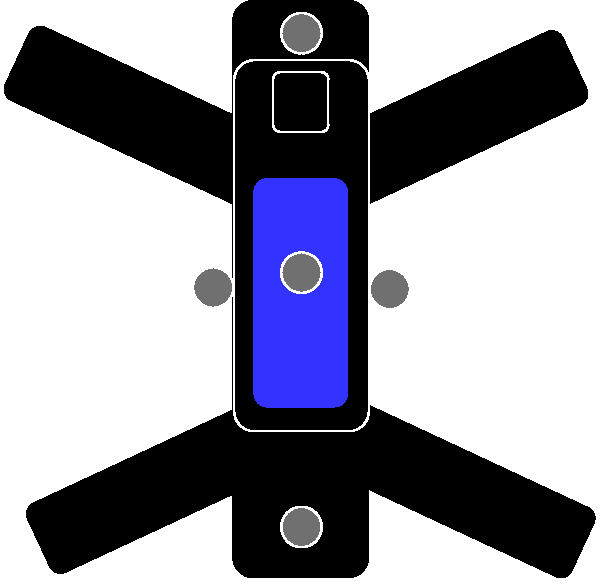
\includegraphics[width=0.4\textwidth]{figures/Appendix/measuringTest/Reflector1.pdf}
    \caption{Illustration of placement of the reflectors on the drone.}
    \label{fig:reflectors_secondary}
\end{figure}

\section*{Execution}
Before the test can be executed, a calibration of the Vicon cameras have to be done. After the Calibration the test code is transferred to the Teensy for controlling the drone. The drone will be manually flown by the pilot up to a height far enough away from the floor where it hovers without the help of the air-cushion it generates close to the ground. This is >400 mm. This is done because the air cushion has an effect on the step response. When the drone is hovering the step can be applied, at this state the drone has a throttle value of 35.1 \%. Then the program is started so the drone will increase the throttle value by 2 \% for one second and after this second the drone will go back to hovering. The whole step response is tracked and recorded using the Vicon system and the reflectors on the drone.


\section*{Results}
From the Vicon system the result from the step response are plotted using Matlab. The plot can be seen on figure \ref{fig:secondary_stepresponse}.
\begin{figure}[H]
    \centering
    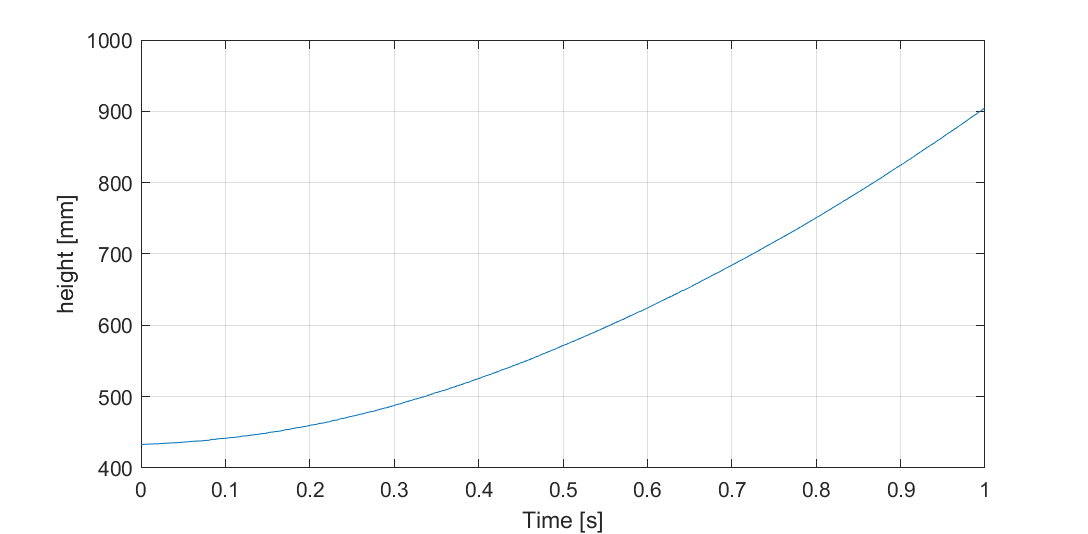
\includegraphics[width=\textwidth]{figures/Appendix/secondary_stepresponse.png}
    \caption{Plot of the step response made using the tracked data from Vicon.}
    \label{fig:secondary_stepresponse}
\end{figure}

From the data it can be seen, that the response is looking more like a first order transfer function, because it has a more linear behavior, which is a fundamental element for a first order transfer function. A first order transfer function is based on the equation \ref{eq:first_order}.
\begin{equation}\label{eq:first_order}
    G(s)=\frac{1}{sT}
\end{equation}
To get the closed loop control system from this equation \ref{eq:first_order}, there are some assumption that needs to be made, first the system has an output C(s) and an input R(s), then the equation \ref{eq:closed_loop_first}.
\begin{equation}\label{eq:closed_loop_first}
    \frac{C(s)}{R(s)}=\frac{G(s)}{1+G(s)} \to \frac{C(s)}{R(s)}= \frac{\frac{1}{sT}}{1+\frac{1}{sT}}=\frac{1}{sT+1}
\end{equation}
This equation is a closed loop transfer function for a first order system \cite{digital_control}. 



















